\documentclass{article}
\usepackage{graphicx}
\usepackage{float}
\usepackage{biblatex}
\usepackage{xurl}
\usepackage{listings}
\usepackage{xcolor}

\definecolor{codegreen}{rgb}{0,0.6,0}
\definecolor{codegray}{rgb}{0.5,0.5,0.5}
\definecolor{codepurple}{rgb}{0.58,0,0.82}
\definecolor{backcolour}{rgb}{0.95,0.95,0.92}

\lstdefinestyle{mystyle}{
    backgroundcolor=\color{backcolour},   
    commentstyle=\color{codegreen},
    keywordstyle=\color{magenta},
    numberstyle=\tiny\color{codegray},
    stringstyle=\color{codepurple},
    basicstyle=\ttfamily\footnotesize,
    breakatwhitespace=false,         
    breaklines=true,                 
    captionpos=b,                    
    keepspaces=true,                 
    numbers=none,                    
    numbersep=5pt,                  
    showspaces=false,                
    showstringspaces=false,
    showtabs=false,                  
    tabsize=2
}

\lstset{style=mystyle}
\addbibresource{ref.bib}
\graphicspath{{./images}}
\title{Analysis of NetWireRAT\\Practical Assignment 4\\Malware Reverse Engineering \\
CAP6137}
\author{Michael Ivanov \\
ivanovmichael@ufl.edu}
\date{April 20, 2022}
\hfuzz=30pt

\begin{document}
    \maketitle
    \pagebreak
    \section{Executive Summary}
    This piece of malware is a \textit{Remote Access Trojan (RAT)} keylogger. Executing this malware will cause the following directory to be created \url{C:\Users\malware\AppData\Roaming\Logs}. Inside this directory files with the current date will be created. These files are encoded to disguise any intent and are updated every time the user presses any keys. Through static and dynamic analysis I was able to find the encoding methods to decode the logged messages. Decoding these files reveals the malware's purpose. The malware records the current active window's name with any keys pressed while the window is in focus. This allows the malware to potentially gather information on any confidential information the user types into a document or browser. Analyzing network traffic reveals two address the malware attempts to connect to: \url{masonchill.jumpingcrab.com} and \url{masonchill.dynamic-dns.net}.
    \pagebreak
    \section{Static Analysis}
    \subsection{MD5 Hashes}
    \begin{itemize}
        \item NetWireRat.exe: 1D7FFEE59EA65A8E19F28BAF72F581F4 \Cite{malwareSample}
    \end{itemize}
    \subsection{Compilation date}
    \begin{itemize}
        \item NetWireRat.exe: Sat Apr 04 14:56:51 2015
    \end{itemize}
    \subsection{Suspicious Imports}
    Libraries
    \begin{itemize}
        \item crypt32.dll
        \item ws2\textunderscore32.dll
    \end{itemize}
    Functions
    \begin{itemize}
        \item \textbf{socket, closesocket, connect, send, gethostname}: Various socket related functions.
        \item \textbf{WriteFile, MoveFileA, DeleteFileA, FindFirstFileA, FindNextFileA}: File operations.
        \item \textbf{RegDeleteKeyA, RegDeleteValueA, RegSetValueA}: registry operations.
        \item \textbf{CryptCreateHash, CryptHashData, CryptDestroyHash}: various cryptographic functions related to hashing.
        \item \textbf{OpenProcess, GetCurrentProcessId, Process32First, Process32next, TerminateProcess} various process related functions.
    \end{itemize}
    \subsection{Suspicious strings}
    \begin{itemize}
        \item \url{@echo off\r\nping 192.0.2.2 -n 1 -w %d >nul 2>&1\r\nDEL /s "%s" >nul 2>&1\r\ncall :deleteSelf&exit /b\r\n:deleteSelf\r\nstart /b "" cmd /c del "%%~f0"&exit /b\r\n}: A shell script.
        \item \url{FCONNECT %s:%d HTTP/1.0\r\nHost: %s:%d\r\n\r\n}
        \item \url{%s\Google\Chrome\User Data\Default\Login Data} a format string with a path to some login data for Google Chrome.
        \item \url{%s\Opera Software\Opera Stable\Login Data}
        \item \url{$s\Chrominum\User Data\Default\Login Data}
        \item \url{%s\Mozilla\SeaMonkey\profiles.ini}
        \item \url{$s\Mozilla\Firefox\profiles.ini}
        \item \url{%s\Opera\Opera\profile\wand.dat}
        \item \url{SOFTWARE\Mozilla\$s\%s\Main}
        \item \url{%s\Thunderbird\profiles.ini}
        \item \url{$s\system32\cmd.exe}
        \item \url{sqlite3 column text}
        \item \url{select * from moz logins}
    \end{itemize}
    \subsection{Program Sections}
    Nothing suspicious found with the program sections.
    \subsection{Anti-disassembly and anti-debugging}
    No anti-disassembly or anti-debugging was found.
    \subsection{Obfuscation}
    \begin{figure}[H]
        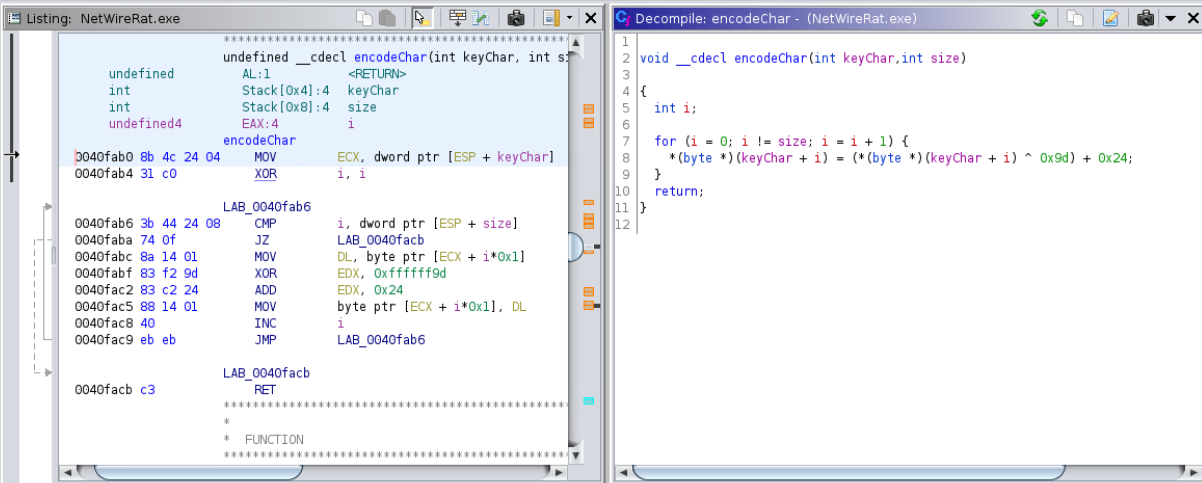
\includegraphics[width=\textwidth]{ghidra-encode.png}
        \caption{The code responsible for encoding the tracked key presses}
        \label{fig:encode}
    \end{figure}
    \subsection{Interesting disassembly functions}
    \begin{figure}[H]
        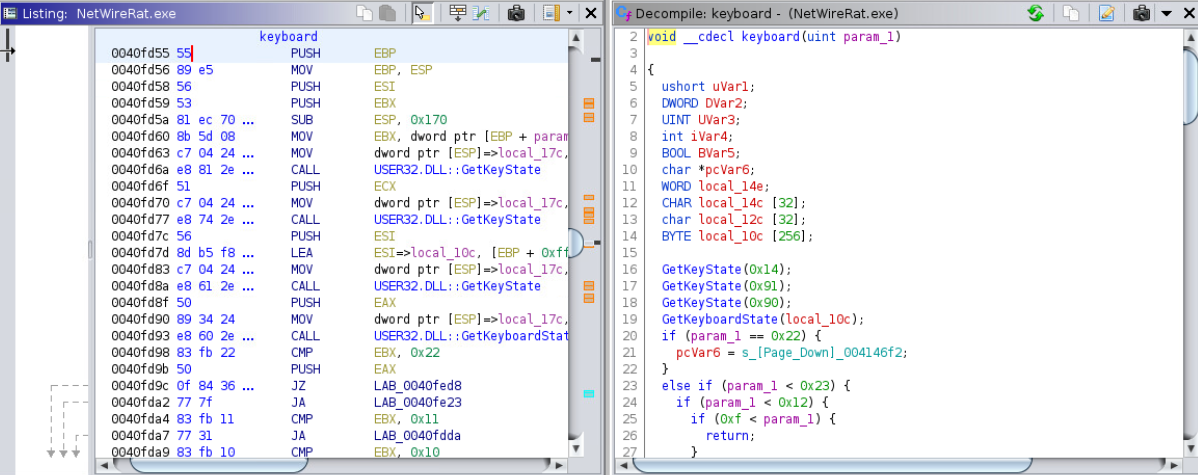
\includegraphics[width=\textwidth]{keyboard-function.png}
        \caption{Ghidra disassembly of where the RAT records key presses}
    \end{figure}
    \begin{figure}[H]
        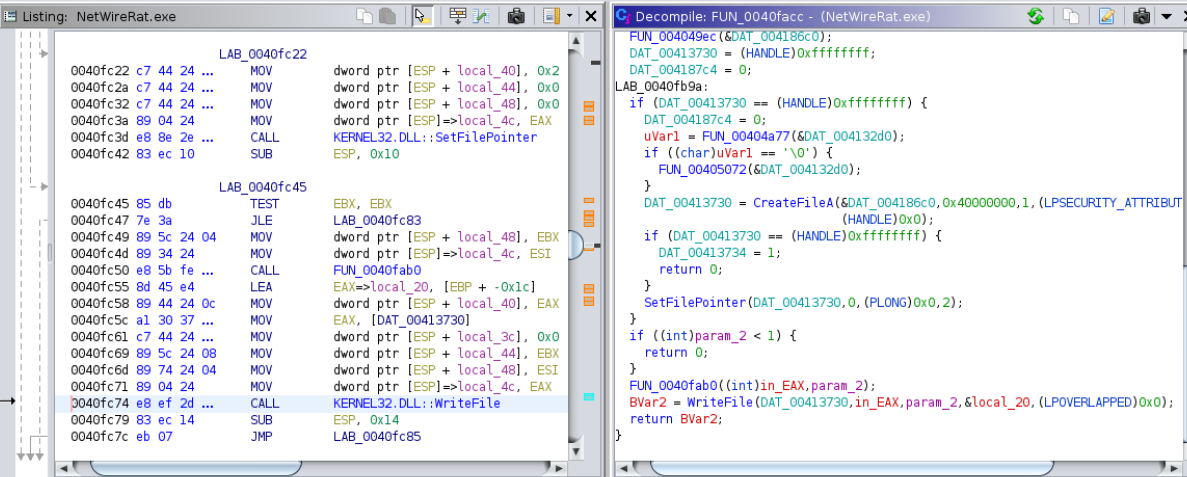
\includegraphics[width=\textwidth]{ghidra-writeFile.png}
        \caption{Ghidra disassembly of where the RAT writes its log}
    \end{figure}
    \pagebreak
    \section{Dynamic Analysis}
    \subsection{Interesting behaviors}
    Executing the malware it will create a Logs directory and a file with the current date. When typing in any application this log file will be updated with encoded data to disguise its purpose.
    \begin{figure}[H]
        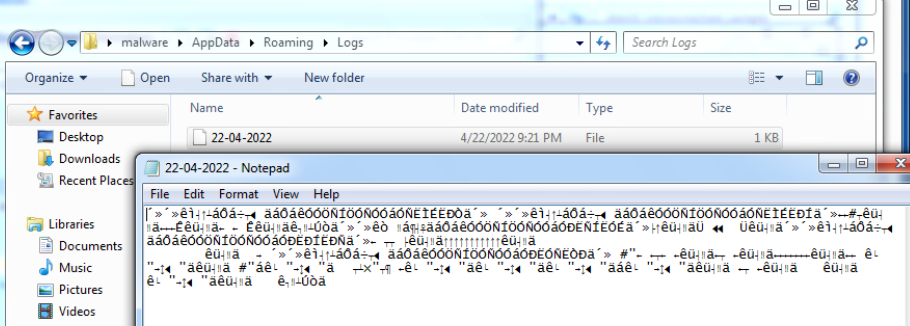
\includegraphics[width=\textwidth]{encoded-logs.png}
        \caption{Encoded data created by the malware}
    \end{figure}
    \begin{figure}[H]
        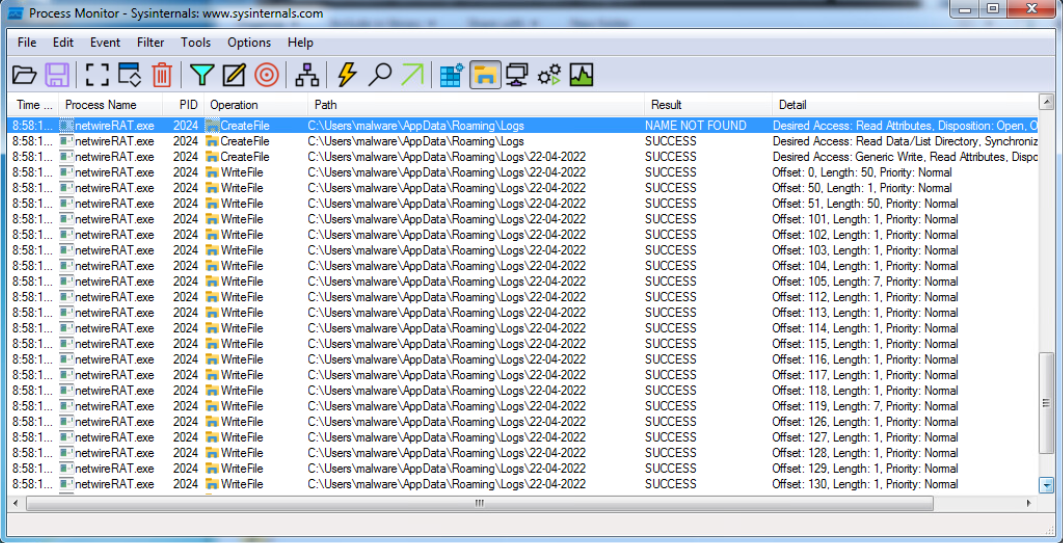
\includegraphics[width=\textwidth]{procmon-logs.png}
        \caption{Procmon showing the creation and modification of the log file}
    \end{figure}
    \pagebreak
    By analyzing the encoding function in figure \ref{fig:encode}, a decoding script can be created to reverse the process.
    \begin{lstlisting}[language=Python]
encodedFile = open('encode.txt', 'r')
decodedFile = open('decode.txt', 'w')
while True:
    c = encodedFile.read(1)
    if not c:
        break
    c = ord(c)
    c -= int(0x24)
    c %= 256
    c ^= int(0x9d)
    decodedFile.write(chr(c))
encodedFile.close()
decodedFile.close()
    \end{lstlisting}
    Executing the script above on the log file gives us the decoded text.     The log contains the active window, the date and time, and any keys pressed.
    \begin{figure}[H]
        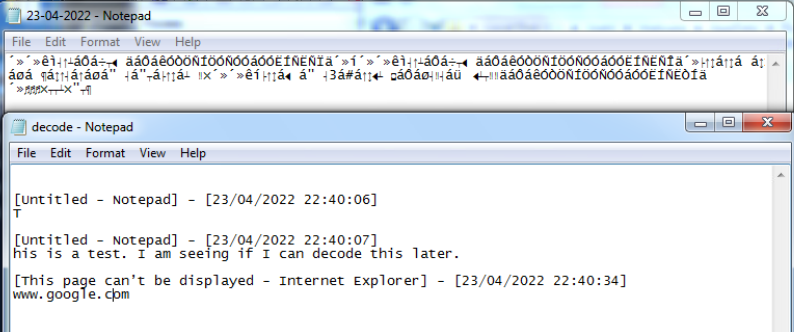
\includegraphics[width=\textwidth]{decoded-logs2.png}
        \caption{The decoded log file after executing the python script}
    \end{figure}
    \begin{figure}[H]
        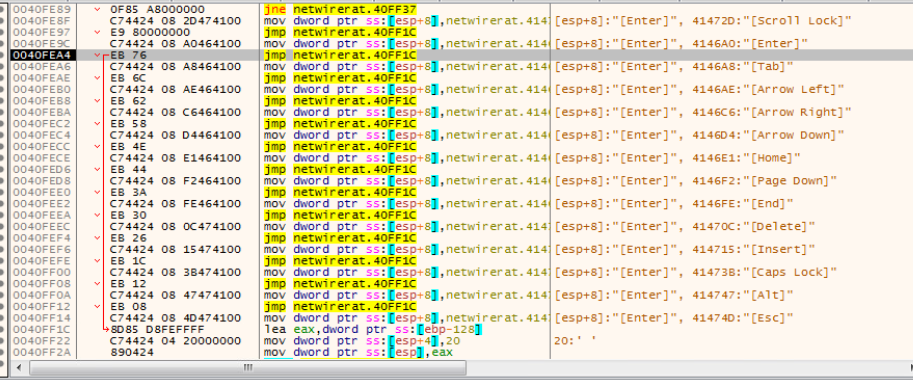
\includegraphics[width=\textwidth]{x32-keys.png}
        \caption{Using x32dbg the malware is shown to look for non-printable keys as well}
    \end{figure}
    \subsection{Networking activity}
    DNS Resolutions:
    \begin{itemize}
        \item \url{masonchill.jumpingcrab.com}
        \item \url{masonchill.dynamic-dns.net}
    \end{itemize}
    \begin{figure}[H]
        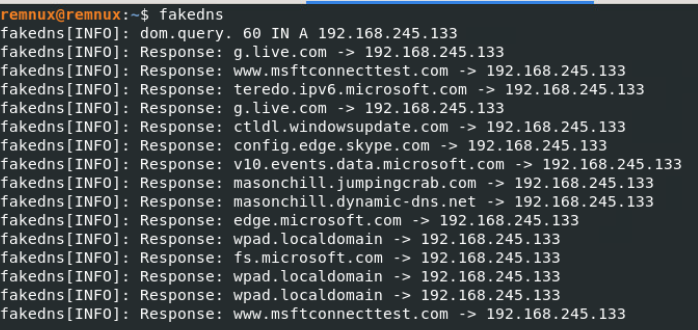
\includegraphics[width=\textwidth]{fakedns.png}
        \caption{Remnux running fakedns while malware is running}
    \end{figure}
    \begin{figure}[H]
        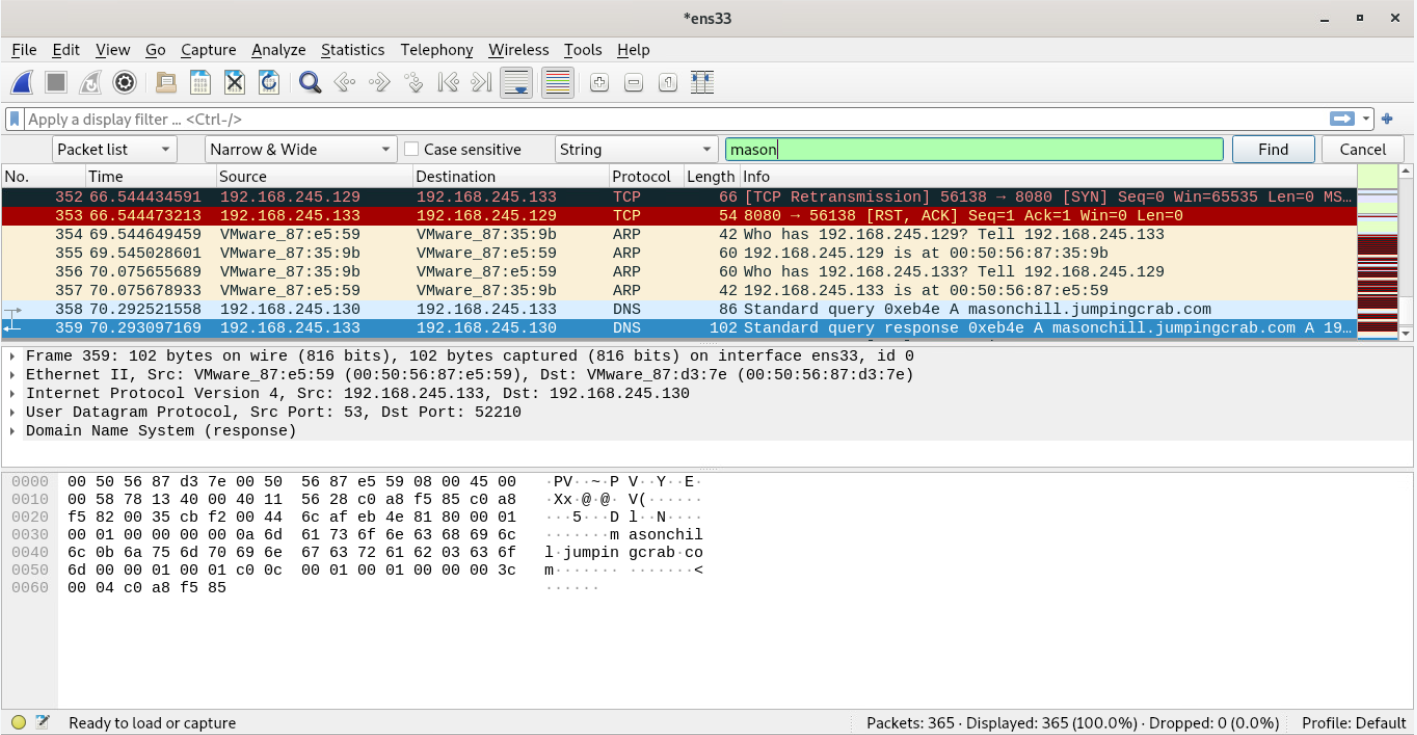
\includegraphics[width=\textwidth]{wireshark.png}
        \caption{DNS response shown in Wireshark}
    \end{figure}
    \subsection{Registry keys created or modified}
    No registry keys were created or modified.
    \subsection{Files created or modified}
    Files and directories created:
    \begin{itemize}
        \item \url{C:\Users\malware\AppData\Roaming\Logs}: directory was created
        \item \url{C:\Users\malware\AppData\Roaming\Logs\20-04-2022}: file with today's date is created and modified multiple times.
    \end{itemize}
    \subsection{Persistence}
    No persistence mechanisms have been observed. The log file persists between reboots, but no longer updates on key presses. Also, network activity stops on reboot as well.
    \pagebreak
    \section{Indicators of Compromise}
    \subsection{Host Indicators}
    The following directory and file:
    \begin{itemize}
        \item \url{C:\Users\malware\AppData\Roaming\Logs}
        \item \url{C:\Users\malware\AppData\Roaming\Logs\%date%}
    \end{itemize}
    \subsection{Network Indicators}
    The following dns resolutions:
    \begin{itemize}
        \item \url{masonchill.jumpingcrab.com}
        \item \url{masonchill.dynamic-dns.net}
    \end{itemize}
    \subsection{Yara Rule}
    \begin{lstlisting}
import "pe"

rule netWireRAT {
    meta:
        author = "Michael Ivanov"
    strings:
        $s1 = "User Data" fullword ascii
        $s2 = "GetRawInputData" fullword ascii
        $s3 = "GetKeyState" fullword ascii
    condition:
    uint16(0) == 0x5A4D
    and $s1 and $s2 and $s3
    and pe.imports("ws2_32.dll") 
    and pe.imports("crypt32.dll") 
    and pe.imports("user32.dll", "EnumWindows") 
    and pe.imports("user32.dll", "GetForegroundWindow") 
    and pe.imports("user32.dll", "GetDesktopWindow")  
}
    \end{lstlisting}
    \pagebreak
    \printbibliography
\end{document}